% % % % % % % % % % % % % % % % % % % % % % % % % % % % % % % % % % % % % % % %
%
% LICENZA
%
% Quest'opera è stata rilasciata sotto la licenza
% Creative Commons Attribution-NonCommercial-ShareAlike 2.5 Italy.
% Per leggere una copia della licenza visita il sito web
% http://creativecommons.org/licenses/by-nc-sa/2.5/it/
% o spedisci una lettera a Creative Commons, 171 Second Street, Suite 300, San
% Francisco, California, 94105, USA.
%
% This work is licensed under the Creative Commons
% Attribution-NonCommercial-ShareAlike 3.0 Unported License. To view a copy of
% this license, visit http://creativecommons.org/licenses/by-nc-sa/3.0/ or send
% a letter to Creative Commons, 171 Second Street, Suite 300, San Francisco,
% California, 94105, USA.
%
% For info send a mail to pietro.giuffri@gmail.com
%
% % % % % % % % % % % % % % % % % % % % % % % % % % % % % % % % % % % % % % % %

\documentclass[a4paper,12pt,oneside]{article}
\usepackage[utf8]{inputenc}
\usepackage[italian]{babel}

\usepackage[font=small,format=hang]{caption}
\usepackage{graphicx}

\usepackage{listings}
\usepackage{fourier}

\usepackage[bookmarks=false,colorlinks=true]{hyperref}
\usepackage{breakurl}
\usepackage{guit}

\lstset{basicstyle=\small\ttfamily,
  keywordstyle=\color{blue},
  commentstyle=\color{red},
  stringstyle=\color{green},
  frame=lines,
  breaklines = true, % per mandare a capo le righe troppo lunghe
  breakautoindent = true, % indenta le righe spezzate
  breakindent = 30pt, % indenta le righe di 30pt
  language=bash,
  showspaces=false,
  showstringspaces=false,
  showtabs=false,
  emph={touch,mkdir,echo,rm,git},
  emphstyle=\color{blue}
}

\begin{document}
\title{git4\LaTeX \\
  Una guida introduttiva a Git per progetti \LaTeX}
\author{Pietro Giuffrida}
\maketitle
\clearpage
\tableofcontents
\clearpage
\section{Scopo della guida}
Git è un \emph{revision control system} (o \emph{version control system}, spesso
abbreviato in VCS), vale a dire un programma che permette di tener traccia di
tutte le modifiche e le evoluzione effettuate nel corso della stesura di un
codice o di un qualsiasi progetto su supporto digitale. Git è rilasciato sotto
licenza GPL, ed è disponibile, oltre che nei repository delle varie distribuzioni
GNU-Linux, all'indirizzo \url{http://git-scm.com/}.

\LaTeX{} è un programma di composizione tipografica di alta qualità. \LaTeX{} è
software libero. Generalmente fa parte dei programmi fondamentali preinstallati in
ogni distribuzione GNU-Linux, ed è comunque disponibile a partire dall'indirizzo
\url{http://www.latex-project.org/} per i principali sistemi operativi.

In questo documento desidero mostrare come utilizzare Git per tener traccia
delle modifiche rilevanti e delle versioni elaborate nel corso dell'elaborazione
di un documento scritto con \LaTeX. Tramite Git è infatti possibile mantenere un
backup incrementale del proprio codice sorgente, sia in locale che in remoto,
senza incorrere in un eccessivo dispendio di energie e senza deconcentrarsi
eccessivamente dalla stesure del proprio testo. I passaggi descritti
relativamente all'uso di Git dovrebbero essere validi in linea di principio per
l'elaborazione di qualsiasi documento (foto, file \lstinline|.doc|, \lstinline|.xls|
e quant'altro), ma Git dà il meglio di sé con i file di testo puro, poiché permette
di vedere tutte le modifiche apportate al file di volta in volta. Proprio per questo
l'uso principale di Git, e dei VCS in generale, è quello di controllare lo sviluppo
dei software.\footnote{Git, infatti, è stato creato da Linus Torvalds, inventore
  del kernel Linux, perché aveva bisogno di un buon VCS per gestire lo sviluppo
  di Linux.} Anche il codice dei documenti \LaTeX{} si scrive su file di testo
puro e quindi Git è particolarmente adatto a essere utilizzato in accoppiata con
\LaTeX. Questa guida è proprio strutturata in modo specifico per illustrare la
loro interazione, almeno a livello base.

Solo i primi due paragrafo sono indispensabili. In essi vengono tratte le basi
del funzionamento di Git e  mostrati i passaggi fondamentali per la creazione di
un repository locale del proprio progetto, per il salvataggio progressivo delle
versioni, e quindi per svolgere eventuali operazioni di ripristino.

I paragrafi successivi sono invece dedicate alla creazione e alla
sincronizzazione di un repository remoto (che si tratti di un servizio on-line
o semplicemente di una memoria esterna), e a uno script bash che permette di
eseguire dei commit automatici a ogni salvataggio dei file.

La guida non si prefigge alcun compito specifico per quanto riguarda \LaTeX, a
proposito del quale esistono numerose guide.\footnote{Si veda a questo proposito,
  oltre alla documentazione reperibile sul proprio computer mediante il comando
  \lstinline|texdoc nomepacchetto|, la documentazione in italiano reperibile a
  partire dal sito del \guit\ (\url{http://www.guit.sssup.it}), oltre all'ottima guida
  di L. Pantieri disponibile sul sito
  \url{http://www.lorenzopantieri.net/LaTeX.html}.}

La guida non contempla l'uso di una qualunque interfaccia grafica (GUI). Tutti i
comandi e i passaggi illustrati sono eseguiti tramite una shell Linux.
Non ho esperienza né di Git né di \LaTeX{} su sistemi operativi non
Unix-like. Un minimo di compatibilità con altri sistemi è garantita dal fatto
che i comandi tipici della shell Linux sono evidenziati e commentati, in modo
che l'utente di altri sistemi operativi o abituato all'uso di GUI possa
sostituirli svolgendo altrimenti le medesime attività. I comandi di
Git dovrebbero invece restare i medesimi in ogni OS, per quanto anche in questo
caso le medesime attività possano essere svolte mediante GUI.

Non sono un esperto di informatica, ma trovo bello far le cose, per quanto
possibile, con le mie mani, sapere cosa fa la macchina e avere l'illusione che
nel rapporto quasi-simbiotico con il computer sia io a decidere.

Dato il carattere ludico della presente guida, scelgo come licenza la Creative
Commons Attribution-NonCommercial-ShareAlike 2.5 Italy. Gli unici vincoli sono
quindi quelli di riconoscere la paternità dell'opera
originale, di non lucrare sulla sua distribuzione, e di distribuire l'opera e
i suoi eventuali derivati con la medesima licenza.\footnote{
  Quest'opera è stata rilasciata sotto la licenza
  Creative Commons Attribution-NonCommercial-ShareAlike 2.5 Italy.
  Per leggere una copia della licenza visita il sito web
  \url{http://creativecommons.org/licenses/by-nc-sa/2.5/it/}
  o spedisci una lettera a Creative Commons, 171 Second Street, Suite 300, San
  Francisco, California, 94105, USA.}

\section{Introduzione a Git}
Git permette di tenere traccia delle modifiche apportate a un progetto registrando
una copia dei file del progetto in un database. Sostanzialmente Git scatta una
foto dei file presenti nella cartella nel momento in cui si effettua il
\emph{commit}.

Per controllare continuamente l'integrità dei dati Git utilizza un sistema, detto
\emph{checksum}, che associa a ogni stato di un progetto una sequenza di bit che
la identifica. Nella fattispecie Git utilizza l'algoritmo SHA-1 che restituisce
una stringa esadecimale (detta \emph{hash}) composta da $40$ caratteri
alfanumerici (numeri da \lstinline|0| a \lstinline|9| e lettere da \lstinline|a|
a \lstinline|f|) che può apparire così:
\begin{lstlisting}
43c5858e91a7090b834dd9f09ddfae1061901ee4
\end{lstlisting}
In questo modo è impossibile modificare un file del progetto senza che Git se
ne renda conto. Per fare riferimento a una particolare versione del progetto
si indica il corrispondente \emph{hash} o, a volte, solo i primi $7$ caratteri.

\begin{figure}
  \centering
  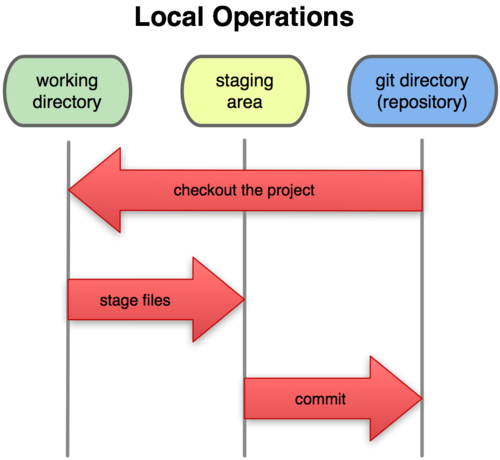
\includegraphics{18333fig0106-tn}
  \caption{Working directory, staging area e git directory. Immagine presa da:
    \url{http://progit.org/book/ch1-3.html}.}
\end{figure}
Prima di iniziare a metterci al lavoro c'è un'ultima cosa da sapere su Git. I
file possono trovarsi in tre stati chiamati, in inglese, \emph{committed},
\emph{modified} e \emph{staged}. \emph{Commited} significa che il file è stato
salvato nel proprio database locale; \emph{modified} indica che il file è stato
modificato ma non ancora salvato nel database con un \emph{commit};
\emph{staged} significa che il file è stato modificato e la sua versione attuale
verrà salvata nel database con il \emph{commit} successivo.
Un progetto Git può quindi essere suddiviso in tre sezioni principali: la
\emph{git directory}, la \emph{working directory} e la \emph{staging area}. La
prima è dove Git conserva i metadati e gli oggetti del database del proprio
progetto. La \emph{working directory} è, come dice il nome stesso, la ``cartella
di lavoro'', ossia una copia di una versione del progetto a nostra disposizione
per l'uso e la modifica dei file. L'ultima sezione, la \emph{staging area}, è un
semplice file, generalmente contenuto nella cartella Git, che conserva le
informazioni su ciò che dovrà entrare nel \emph{commit} successivo.

Con Git si lavora più o meno così:
\begin{enumerate}
\item si modifica un file presente nella \emph{working directory};
\item si aggiunge un suo \emph{snapshot}, cioè una sua copia, nella \emph{staging
    area};
\item si esegue un \emph{commit}, cioè l'operazione con la quale i file vengono
  copiati così come sono presenti alla \emph{staging area} all'interno della
  git directory in maniera definitiva. Al \emph{commit} viene associato
  l'\emph{hash} che identifica univocamente la versione del progetto così salvata.
\end{enumerate}
Se una particolare versione di un file si trova nella cartella git è considerato
\emph{committed}. Se è stato modificato e aggiunto alla \emph{staging area} esso
è detto \emph{staged}. Se è stato modificato da quando è stata aperta la cartella
di lavoro ma non ancora aggiunto alla \emph{staging area} allora il file è detto
\emph{modified}.\footnote{Questo paragrafo è stato tradotto in parte da
  \url{http://progit.org/book/ch1-3.html}.}

\section{Un semplice progetto \LaTeX}
Vogliamo sviluppare un documento con \LaTeX, utilizzando Git come VCS.
Git non funziona in modo particolarmente esotico. Si tratta semplicemente di
creare una directory, di posizionare in essa i nostri file \lstinline|.tex| e di
dire a Git di considerare tale directory come un repository.
\subsection{Creazione e inizializzazione del repository}
\begin{lstlisting}
~$ mkdir progetto
~$ cd progetto
~/progetto$ touch np_main.tex
~/progetto$ git init
~/progetto$ git add .
~/progetto$ git commit -am "Inizializzazione del nuovo progetto"
\end{lstlisting}
Vediamo con calma i singoli passaggi. I primi tre comandi servono
rispettivamente per creare la directory (\lstinline|mkdir nome_directory|),
per spostarsi al suo interno (\lstinline|cd nome_directory|) e per creare
un file vuoto chiamato \lstinline|np_main.tex| (\lstinline|touch nome_file|).

I passaggi successivi, eseguiti sempre dati dall'interno della directory, sono
quelli specifici di Git:
\begin{itemize}
\item con \lstinline|git init| creiamo una cartella nascosta chiamata
  \lstinline|.git/| che contiene il nostro repository Git;
\item \lstinline|git add .| aggiunge l'argomento (in questo caso `\lstinline|.|',
  ossia la cartella in cui siamo posizionati e tutti i file al suo interno) alla
  \emph{staging area} del repository appena creato;
\item con col comando \lstinline|commit -am "nota di versione"| effettuiamo il
  commit che, come detto, salva una copia dei file contenuti nella \emph{staging
    area} all'interno del database. Nel registro delle operazioni effettuate a
  questa operazione risulterà associato il messaggio \lstinline|"nota di versione"|.
\end{itemize}

Così facendo saremo già pronti a lavorare con il nostro editor di fiducia sul
file \lstinline|.tex| appena creato.
Non resta che eseguire un \emph{commit} al termine di ogni modifica rilevante,
in modo da salvare una determinata versione del progetto.
\begin{lstlisting}
~/progetto$ echo "una modifica rilevante" >> np_main.tex
~/progetto$ git commit -am "ulteriore sviluppo"
\end{lstlisting}

Finora abbiamo eseguito il \emph{commit} passando a Git le due opzioni
\lstinline|-am|. Con l'opzione \lstinline|-m| diciamo a Git di utilizzare il
testo tra virgolette che segue il comando come nota di versione del \emph{commit}
che stiamo eseguendo. Con l'opzione \lstinline|-a| chiediamo a Git di mettere
nella \emph{staging area} tutti i file del progetto prima di eseguire il
\emph{commit}. Se non specifichiamo un messaggio con l'opzione \lstinline|-m| si
aprirà l'editor di testo associato di default a Git in cui potremo scrivere il
messaggio del \emph{commit}. Vedremo più avanti come impostare l'editor.

\subsection{Aggiungere altri file al progetto: il file \lstinline|.gitignore|}
Si presenta ora uno scenario tra i più comuni: dobbiamo aggiungere un ulteriore
file al progetto, per esempio un file \lstinline|.tex| contenente un ulteriore
capitolo, o un file \lstinline|.bib| contenente la bibliografia, o un qualsiasi
altro file. Quando eseguiamo il \emph{commit} successivo, potremmo aspettarci
che Git si accorga del nuovo arrivato, e in effetti dovrebbe restituire un
messaggio di questo tipo:
\begin{lstlisting}
~/progetto$ touch np_secondary.tex
~/progetto$ git commit -am "aggiunto file np_secondary.tex"
# On branch master
# Untracked files:
#   (use "git add <file>..." to include in what will be committed)
#
#       np_secondary.tex
nothing added to commit but untracked files present (use "git add" to track)
\end{lstlisting}
Git si accorge quindi della presenza di un nuovo file, ma non lo aggiunge
automaticamente al progetto. D'altra parte, se avesse rilevato delle modifiche
ai file precedentemente aggiunti al progetto, non si sarebbe nemmeno curato di
comunicarci che il nuovo file non è ancora stato aggiunto al progetto. Si
sarebbe infatti limitato a salvare le modifiche ai file che gli abbiamo
precedentemente detto di gestire. Solo con il comando \lstinline|git status|
Git ci comunica con certezza l'anomalia di un nuovo file non ancora caricato nel
repository.

Git è un programma molto gentile perché ci dà spesso dei suggerimenti molto utili.
Infatti se osserviamo attentamente l'output precedente possiamo vedere che Git
ci sta dicendo che possiamo includere i nuovi file con il comando
\begin{lstlisting}
git add <file>...
\end{lstlisting}
Si può scegliere di procedere in due modi:
aggiungere indiscriminatamente tutti i file della directory al progetto che
stiamo sviluppando; oppure aggiungere un singolo file. Nel primo caso dovremmo
ripetere il comando già usato in fase di inizializzazione:
\begin{lstlisting}
~/progetto$ git add .
\end{lstlisting}
Nel secondo caso aggiungiamo un singolo file:
\begin{lstlisting}
~/progetto$ git add np_secondary.tex
\end{lstlisting}

Per quanto possa sembrare eccessivo, io preferisco usare il secondo comando.
Mi accade con estrema frequenza di
dover aggiungere dei file a un progetto, e spesso sono fin troppo
distratto da quel che sto scrivendo per occuparmi di quel Git si aspetta da me
L'aggiunta indiscriminata di ogni file nella directory al repository presenta
però delle controindicazioni.
La più ovvia per chi lavora con \LaTeX{} è la seguente:
nel corso dell'elaborazione di un testo inevitabilmente si
procederà alla generazione del documento in pdf a partire dai sorgenti;
\LaTeX{} provvederà quindi alla generazioni di una serie di file secondary
(\lstinline|.toc|, \lstinline|.out|, \dots), nonché di un pdf più o meno inutile.
Se eseguissimo il comando \lstinline|git add .| subito dopo una compilazione,
evidentemente Git aggiungerebbe alla \emph{staging area} anche i vari file di
lavoro, dal pdf, ai file  di log. Per ovviare a questo inconveniente, e continuare
pigramente a eseguire \lstinline|git add .|, è utile creare nella nostra
directory di un file denominato \lstinline|.gitignore|.
\begin{lstlisting}
~/progetto$ echo "*.log" >> .gitignore
~/progetto$ echo "*.pdf" >> .gitignore
~/progetto$ echo "*.blg" >> .gitignore
~/progetto$ echo "*.bbl" >> .gitignore
~/progetto$ echo "*.aux" >> .gitignore
~/progetto$ echo "*-blx.bib" >> .gitignore
~/progetto$ echo "*.out" >> .gitignore
~/progetto$ echo "*~" >> .gitignore
~/progetto$ git add .gitignore
~/progetto$ git commit -am "Aggiunto il file .gitignore"
\end{lstlisting}

Mediante questo file, istruiamo Git a proposito di tutti i file che non fanno
effettivamente parte del progetto, pur essendo presenti nella cartella.
Da questo momento in poi Git si limiterà a ignorarli, il che ci permette di
eseguire prudenzialmente il comando \lstinline|git add .| prima di ogni
\emph{commit}.

\subsection{Consultazione dei log e ripristino di file}
Ipotizziamo a titolo esemplificativo il seguente scenario:
abbiamo accidentalmente eliminato un file del nostro
progetto, e abbiamo anche eseguito un \emph{commit}.
\begin{lstlisting}
~/progetto$ echo "pippo" >> np_secondary.tex
~/progetto$ git add .
~/progetto$ git commit -am "Ho solo iniziato a lavorare"
~/progetto$ rm np_secondary.tex
~/progetto$ git commit -am "Ma ho gia' perso tutto"
\end{lstlisting}

Ora chiediamo conto a Git della sua capacità di ripristinare una versione
precedentemente salvata. La prima cosa da fare è consultare i log dei commit
precedentemente effettuati, per decidere quale di essi ripristinare. Il comando
appropriato sarebbe quindi \lstinline|git log|, che contempla anche un'ampia
serie di interessanti opzioni. Rimandando al manuale per la maggior parte di tali
opzioni, segnalo solo che è possibile:
\begin{itemize}
\item selezionare esclusivamente i log relativi a un dato file, con la
  sintassi \lstinline|git log nome_file|;
\item chiedere a Git di stampare solo gli ultimi $n$ log, con la
  sintassi \lstinline|git log -n|.
\end{itemize}
Trattandosi di un file eliminato, non possiamo chiedere a Git di stampare solo i
log a esso relativi. Dobbiamo quindi cercare tra i log più recenti fino a
identificare uno stadio del progetto in cui il file è ancora presente.
\begin{lstlisting}
~/progetto$ git log -2
commit 380228784f4095efdbce9d1d3408bcbdf01548cb
Author: Pietro Giuffrida <pietro.giuffri@gmail.com>
Date:   Sat Oct 2 18:58:44 2010 +0200

    Ma ho gia' perso tutto

commit c21d825df42f55ba127487fd93acf1c13c41b028
Author: Pietro Giuffrida <pietro.giuffri@gmail.com>
Date:   Sat Oct 2 18:55:07 2010 +0200

    Ho solo iniziato a lavorare
\end{lstlisting}
Nel nostro caso, l'eliminazione del file è ben documentata dalle note.
La lunga stringa che compare dopo \lstinline|commit| è l'\emph{hash} che, come
anticipato prima, è la stringa che identifica univocamente una particolare
versione del progetto. Possiamo subito verificare il contenuto del \emph{commit}
facendo riferimento al corrispettivo \emph{hash} con il comando
\lstinline[language={}]|git show <hash>|:
\begin{lstlisting}
~/progetto$ git show c21d825df42f55ba127487fd93acf1c13c41b028
commit c21d825df42f55ba127487fd93acf1c13c41b028
Author: Pietro Giuffrida <pietro.giuffri@gmail.com>
Date:   Sat Oct 2 18:58:29 2010 +0200

    aggiunto file np_secondary.tex

diff --git a/np_secondary.tex b/np_secondary.tex
new file mode 100644
index 0000000..bfa5424
--- /dev/null
+++ b/np_secondary.tex
@@ -0,0 +1 @@
+pippo
\end{lstlisting}
Il file \lstinline|np_secondary.tex| fa effettivamente parte del commit da noi
individuato. Esso è identificato da un'ulteriore stringa alfanumerica
denominata \emph{index}. Git, tramite il comando \lstinline|diff|, ci comunica
inoltre che esso contiene la stringa \lstinline|pippo|.
Possiamo quindi procedere a ricrearne una copia facendo riferimento
all'\emph{index}:
\begin{lstlisting}
~/progetto$ git show bfa5424 > file_ripristinato
\end{lstlisting}

La procedura, con le complicazioni del caso, dovrebbe essere valida anche per
circostanze concrete. Vi consiglio comunque di fare delle prove simulando per
esempio \emph{commit} di più file contenenti varie modifiche, per far pratica
con gli indici e la sintassi di Git.
Possiamo ipotizzare in questo caso uno scenario di questo tipo:
\begin{lstlisting}
~/progetto$ touch topolino pippo
~/progetto$ echo qualcosa >> topolino
~/progetto$ echo qualcosaltro >> pippo
~/progetto$ git add .
~/progetto$ git commit -am "creati e modificati topolino e pippo"
~/progetto$ echo "ancora qualcosa" >> topolino
~/progetto$ git commit -am "ulteriormente elaborato topolino"
~/progetto$ git log topolino
commit 87548d4cd43cda917cf788866abd76f8399b639b
Author: Pietro Giuffrida <pietro.giuffri@gmail.com>
Date:   Sat Oct 2 19:27:23 2010 +0200

    ulteriormente elaborato topolino

commit f7a696e891bb81446f56adc996bc0a20a23ae9b5
Author: Pietro Giuffrida <pietro.giuffri@gmail.com>
Date:   Sat Oct 2 19:27:01 2010 +0200

    creati e modificati topolino e pippo

~/progetto$ git show f7a696e891bb81446f56adc996bc0a20a23ae9b5
commit f7a696e891bb81446f56adc996bc0a20a23ae9b5
Author: Pietro Giuffrida <pietro.giuffri@gmail.com>
Date:   Sat Oct 2 19:27:01 2010 +0200

    creati e modificati topolino e pippo

diff --git a/pippo b/pippo
new file mode 100644
index 0000000..a09d8a1
--- /dev/null
+++ b/pippo
@@ -0,0 +1 @@
+qualcosa
diff --git a/topolino b/topolino
new file mode 100644
index 0000000..a09d8a1
--- /dev/null
+++ b/topolino
@@ -0,0 +1 @@
+qualcosaltro

~/progetto$ git show a09d8a1 > topolino_ripristinato
\end{lstlisting}

Chiaramente, Git permette il ripristino esclusivamente dei file aggiunti al
repository ed esclusivamente di versioni esplicitamente salvate mediante il
comando \lstinline|commit|. I salvataggi effettuati tra un \emph{commit} e
l'altro non sono quindi ricostruibili.

Nel caso in cui stiamo modificando un file, per esempio
\lstinline|topolino|, ma ci rendiamo conto che le modifiche apportate non ci
soddisfano e vogliamo ripristinarlo alla versione del file salvata nell'ultimo
\emph{commit}, se il file è \emph{modified} ma non \emph{staged}, usando la
terminologia vista all'inizio, possiamo usare il comando \lstinline|checkout|:
\begin{lstlisting}
git checkout topolino
\end{lstlisting}

\subsection{Gestione dei \emph{branch}}
Con il comando \lstinline|git status| possiamo controllare lo stato del progetto,
per esempio se ci sono dei file che sono stati modificati ma non ancora salvati
nel \emph{commit} e così via. Un tipico output di questo comando è:
\begin{lstlisting}
$ git status
# On branch master
nothing to commit (working directory clean)
\end{lstlisting}
All'ultimo rigo leggiamo \lstinline|nothing to commit (working directory clean)|,
cioè non sono presenti file modificati (a parte eventualmente quelli ignorati con
il file \lstinline|.gitignore|) dopo l'ultimo \emph{commit}. Ma cosa significa
\lstinline|On branch master|? \emph{Branch} in inglese significa ``ramo'' e
Git ci dà la possibilità di creare una linea di sviluppo per il nostro progetto
parallela a quella iniziale (chiamata \emph{master} in Git) ma con delle
modifiche che divergono da questa proprio come il ramo di un albero diverge dal
tronco centrale (e per completare questa analogia botanica la linea di sviluppo
centrale è chiamata a volte \emph{trunk}, cioè ``tronco'').

\subsubsection{Perché creare un \emph{branch}?}
Le risposte a questa domanda possono essere diverse. Una potrebbe essere, per
esempio perché abbiamo intenzione di scrivere un capitolo per il nostro documento
\LaTeX{} ma non siamo sicuri che sia veramente necessario: possiamo allora creare
un \emph{branch} nel quale scriveremo solo questo capitolo mentre nel ramo
principale \emph{master} continueremo normalmente a modificare il documento.
Quando il capitolo sarà pronto, se il risultato sarà soddisfacente potremo
procedere alla funsione del ramo ``sperimentale'' in quello principale, operazione
chiamata \emph{merge} in gergo, e nel nostro documento ``comparirà magicamente''
il capitolo che abbiamo sviluppato nel \emph{branch}, in caso contrario possiamo
semplicemente cancellare il \emph{branch}, come se avessimo potato il ramo
indesiderato dell'albero.

Un altro caso in cui può essere utile creare un \emph{branch} è quello in cui si
lavori a più mani su un documento: mentre voi scrivete il vostro documento un
vostro amico vi chiede di collaborarvi (e anch'egli userà Git per tenere traccia
delle sue modifiche). Lui si creerà un suo ramo di sviluppo in modo che voi
potrete continuare a redigere il vostro documento senza che le sue modifiche
vadano a confliggere con le vostre. Alla fine il vostro amico vi farà vedere il
risultato delle sue modifiche: se le apprezzate potete effettuare il \emph{merge}
del suo ramo nel vostro, altrimenti potete dirgli che le sue modifiche non vi
piacciono e il suo \emph{branch} sarà cancellato.\footnote{Il vostro (forse ormai
  ex) amico potrebbe anche decidere di continuare a sviluppare il suo
  \emph{branch} in maniera completamente indipendente da voi: questa situazione,
  nel mondo della programmazione, è detta \emph{fork}.}

Un semplice grafico dello sviluppo di un progetto in cui è stato effettuato un
\emph{branching} potrebbe avere questo aspetto:
\begin{lstlisting}
      E---F---G branch
     /         \
A---B---C---D---H master
\end{lstlisting}
Nel ramo \lstinline|master| abbiamo effettuato le modifiche indicate con
\lstinline|A| e \lstinline|B|. A questo punto creiamo il ramo
\lstinline|branch|. D'ora in poi le modifiche effettuate su un ramo avranno
valore solo su quello: così continuiamo a lavorare normalmente sul ramo
\lstinline|master| apportando le modifiche indicate con \lstinline|C| e
\lstinline|D|, mentre in \lstinline|branch| avremo effettuato le modifiche
\lstinline|E|, \lstinline|F| e \lstinline|G| che apparterranno solo a questo ramo.
Decidiamo quindi di fondere i due rami perché le modifiche fatte in
\lstinline|branch| ci soddisfano: con la modifica \lstinline|H| tutte le modifiche
effettuate in \lstinline|branch| verranno importate nel ramo principale e potremo
continuare lì il nostro lavoro.

\subsubsection{Creare e cancellare un \emph{branch}}
Per creare un \emph{branch} dobbiamo usare il comando
\lstinline|git branch <nome_branch>|. Se il comando va a buon fine non ci sarà
nessun output, possiamo però controllare l'elenco dei rami esistenti con il comando
\lstinline|git branch| senza alcun ulteriore argomento:
\begin{lstlisting}
$ git branch foo
$ git branch
  foo
* master
\end{lstlisting}
L'asterisco vicino a \lstinline|master| sta a indicare che al momento ci troviamo
nel \emph{branch} \lstinline|master|. Per spostarci in un altro \emph{branch}
usiamo il comando \lstinline|git checkout <nome_branch>|:
\begin{lstlisting}
$ git checkout foo
Switched to branch 'foo'
$ git branch 
* foo
  master
\end{lstlisting}
Che significa che ci siamo spostati in un altro \emph{branch}? Abbiamo cambiato
cartella? No, siamo sempre nella stessa cartella (possiamo controllarlo con il
comand \lstinline|pwd|), ma è stato Git che ha modificato la nostra cartella di
lavoro, la \emph{working directory}, andando a prendere dal suo database l'ultimo
\emph{snapshot}, l'ultima ``fotografia'', del \emph{branch} che gli abbiamo
richiesto. In alternativa a \lstinline|git checkout <nome_branch>|, per creare
un nuovo ramo si può usare il comando \lstinline|git checkout -b <nome_branch>|
che in più effettua direttamente il \emph{checkout} del nuovo \emph{branch}:
\begin{lstlisting}
$ git checkout -b foo
Switched to a new branch 'foo'
\end{lstlisting}

Un \emph{branch} appena creato e non modificato è uguale al ramo da cui è stato
creato, contiene i suoi stessi file e la stessa cronologia. Lo sviluppo del progetto
può continuare in maniera identica a quella vista prima (cioè si usano i soliti
comandi \lstinline|git add| e \lstinline|git commit|), però le modifiche apportate
in questo \emph{branch} non compariranno nel registro di quello principale. Possiamo
verificarlo controllando i rispettivi log:
\begin{lstlisting}
$ git branch 
* foo
  master
$ git log 
commit c71da4fe9bf764274e67a2326ec1dc3911691928
Author: Pietro Giuffrida <pietro.giuffri@gmail.com>
Date:   Sat Oct 9 19:09:56 2010 +0200

    primo commit nel branch `foo'

commit e17384278acadbfefefebf0ced4e7103005a597c
Author: Pietro Giuffrida <pietro.giuffri@gmail.com>
Date:   Sat Oct 9 19:08:46 2010 +0200

    iniziamo il nuovo progetto
$ git checkout master 
Switched to branch 'master'
$ git log 
commit e17384278acadbfefefebf0ced4e7103005a597c
Author: Pietro Giuffrida <pietro.giuffri@gmail.com>
Date:   Sat Oct 9 19:08:46 2010 +0200

    iniziamo il nuovo progetto
\end{lstlisting}

Per cancellare un ramo di cui si è già effettuato il \emph{merge} con il ramo
principale (vedremo più avanti come si fa) si usa l'opzione \lstinline|-d| del
comando \lstinline|git branch|:
\begin{lstlisting}
$ git branch -d foo 
Deleted branch foo (was c71da4f).
\end{lstlisting}
Se proviamo a usare l'opzione \lstinline|-d| con un ramo di cui non è stato
ancora effettuato il \emph{merge} Git ci avverte:
\begin{lstlisting}
$ git branch -d foo
error: The branch foo' is not fully merged.
If you are sure you want to delete it, run 'git branch -D foo'.
\end{lstlisting}
Come al solito Git ci suggerisce i comandi che ci possono tornare utili: se
vogliamo ugualmente cancellare il \emph{branch} che non è stato fuso in quello
principale dobbiamo usare l'opzione \lstinline|-D| al posto di \lstinline|-d|:
\begin{lstlisting}
$ git branch -D foo 
Deleted branch foo (was c71da4f).
\end{lstlisting}

\subsubsection{Effettuare un \emph{merge}}
Per effettuare la fusione, \emph{merge}, di due rami si usa il comando
\lstinline|git merge <nome_branch>| da dare nel ramo in cui si desidera importare
il ramo chiamato \lstinline|<nome_branch>|. Se tutto va bene otterremo un output
simile al seguente (supponiamo, per esempio, che il ramo da importare si chiami
\lstinline|foo|):
\begin{lstlisting}
$ git merge foo 
Updating da45d11..729129c
Fast-forward
 capitolo5.tex |   18 ++++++++++++++++++
 1 files changed, 18 insertions(+), 0 deletions(-)
 create mode 100644 capitolo5.tex
\end{lstlisting}
Dopo di ciò possiamo normalmente fare il \emph{commit} con
\lstinline|git add .| e \lstinline|git commit -am "messaggio di commit"|.

Può verificarsi un problema se uno o più file sono stati modificati nello stesso
punto in tutti e due i rami che si vogliono fondere, dopo che è stato creato il
\emph{branch}. Git, infatti, non è in grado di gestire automaticamente questa
situazione (è uno strumento potente ma non può certo leggere nel nostro pensiero,
non può sapere perché il file è stato modificato diversamente nei due rami) e ci
avverte con un messaggio di questo tipo:
\begin{lstlisting}[language={}]
$ git merge foo 
Auto-merging main.tex
CONFLICT (content): Merge conflict in main.tex
Automatic merge failed; fix conflicts and then commit the result.
\end{lstlisting}
In questo caso il file in cui si sono verificati i conflitti si chiama
\lstinline|main.tex|. Aprendo con il nostro editor di testo potremo leggere
a un certo punto qualcosa di questo tipo:
\begin{lstlisting}[language={},emph={HEAD,foo}]
<<<<<<< HEAD
\usepackage{hyperref}
=======
\usepackage[bookmarks=false,colorlinks=true]{hyperref}
>>>>>>> foo
\end{lstlisting}
La zona compresa fra \lstinline|<<<<<<< HEAD| e \lstinline|=======| indica il
contenuto attuale del ramo, mentre ciò che è scritto fra \lstinline|=======| e
\lstinline|>>>>>>> foo| è ciò che si trova nel corrispondente punto dello stesso
file \lstinline|main.tex| ma nel ramo \lstinline|foo|. Dopo aver corretto il file
come desideriamo che risulti, possiamo finalmente salvarlo ed effettuare come al
solito il \emph{commit}.

\subsubsection{Copiare un singolo \emph{commit} da un \emph{branch} a un altro}
Mentre sviluppiamo un \emph{branch} potremmo accorgerci che il \emph{commit} appena
effettuato apporta delle modifiche che possono essere utili anche in un altro
\emph{branch} (come per esempio la correzione di un errore di ortografia o una
modifica al preambolo del documento). Non è necessario effettuare il \emph{merge}
solo per un importare un \emph{commit} o modificare manualmente i file dell'altro
\emph{branch} perché è possibile effettuare un'operazione detta
\emph{cherry-picking} (che significa ``raccolta di ciligie''\footnote{Chi ha
  inventato tutta questa terminologia doveva essere un amante della natura.}) che
nell'importare nell'altro \emph{branch} il singolo \emph{commit} che
indicheremo. La sintassi è semplice (ovviamente prima di dare il seguente comando
bisogna posizionarsi nel \emph{branch} in cui si intende importare il \emph{commit}):
\lstinline|git cherry-pick <hash_del_commit>|. Inoltre l'oggetto, l'autore (nel
caso in cui ci siano più collaboratori che partecipano al progetto) e la data e
orario del \emph{commit} saranno gli stessi di quello importato. Al posto
dell'intero \emph{hash} del \emph{commit} si possono inserire anche solo i primi
$7$ caratteri.

Se dovesse verificarsi qualche problema durante il \emph{cherry-picking}, come
può succedere durante il \emph{merge}, Git ci avverte, ci consiglia di risolvere
i conflitti, usare il solito \lstinline|git add| come opportuno e poi, per
effettuare il \emph{commit}, di dare il comando
\lstinline|git commit -c <hash_del_commit>|, in modo da utilizzare le stesse
informazioni del \emph{commit} a cui ci riferiamo (autore, data e orario,
oggetto):
\begin{lstlisting}[language={},emph=git]
$ git cherry-pick 97b8c9b
Automatic cherry-pick failed.  After resolving the conflicts,
mark the corrected paths with 'git add <paths>' or 'git rm <paths>'
and commit the result with: 

        git commit -c 97b8c9b
\end{lstlisting}

\subsection{Configurazioni basilari di Git}
Per quanto non strettamente indispensabile per un uso individuale di Git sul
proprio pc, segnalo alcune configurazioni elementari necessarie per un uso
ottimale di Git.

Le impostazioni di Git possono essere impostate con il comando
\lstinline|config| di Git. Usando l'opzione \lstinline|--system| le configurazioni
così impostate saranno valide per tutti gli utenti che hanno accesso al sistema
e verranno generalmente salvate nel file di configurazione
\lstinline|$(prefix)/etc/gitconfig|. Con l'opzione \lstinline|--global| le impostazioni
saranno valide solo per il proprio utente e verranno salvate nel file
\lstinline|~/.gitconfig|. Infine non usando alcuna opzione le configurazioni
avranno valore solo per il repository in cui vengono impostate.

In primo luogo occorre passare a Git qualche informazione circa l'utente:
\begin{lstlisting}
git config --global user.name "Pietro Giuffrida"
git config --global user.email pietro.giuffri@gmail.com
\end{lstlisting}
In secondo luogo è utile dire a Git di colorare i log, in modo da renderli più
leggibili:
\begin{lstlisting}
git config --global color.branch auto
git config --global color.diff auto
git config --global color.interactive auto
git config --global color.status auto
\end{lstlisting}
Possiamo poi impostare l'editor di testo predefinito da associre a Git con
l'opzione \lstinline|core.editor|. Se per esempio vogliamo usare Gedit daremo
il comando
\begin{lstlisting}
git config --global core.editor gedit
\end{lstlisting}

\section{Backup}
\subsection{Backup su periferica esterna (usb)}
\begin{lstlisting}
~/progetto$ git clone -l file:///home/pietro/elab/git4latex/ /media/usb/gigt/
\end{lstlisting}

\subsection{Backup on-line}

\begin{enumerate}
\item registrarsi su gitorius (richiede ssh key e passphrase!)
\item \lstinline|git remote add origin git@gitorious.org:git4latex/git4latex.git|
  (che chiederà la passphrase!)
\item \lstinline|git push origin master|
  per sincronizzare il tutto di volta in volta a fine giornata
\end{enumerate}

Prima sincronizzazione da locale verso gitorius:
\begin{lstlisting}
$ git remote add origin git@gitorious.org:progetto/progetto.git
\end{lstlisting}

A fine giornata di lavoro:
\begin{lstlisting}
$ git push origin master
\end{lstlisting}

Se volete ricreare il repository in locale:
\begin{lstlisting}
$ mkdir riprogetto
$ cd riprogetto
$ git clone git://gitorious.org/git4latex/git4latex.git
\end{lstlisting}

\section{commit automatico: inotifywait}

\begin{lstlisting}
inotifywait -q -m -e CLOSE_WRITE --format="git commit -m 'autocommit on change' %w" file.txt | sh
\end{lstlisting}

\begin{lstlisting}
#!/bin/bash
#
# gitwait - watch file and git commit all changes as they happen
#

while true; do

    inotifywait -qq -e CLOSE_WRITE ~/.calendar/calendar

    cd ~/.calendar; git commit -a -m 'autocommit on change'

done
\end{lstlisting}
ma è quasi pericoloso se salvi automaticamente ogni tot minuti!!

\section{Installazione per Windows}
\label{sec:gitwin}

Installare Git su un sistema operativo Windows è davvero molto
semplice. Il progetto \textsf{msysGit} ha una delle più semplici
procedure di installazione.

Bisogna semplicemente scaricare e fare il download dell'installer
\textsf{.exe} dalla pagina
\href{http://code.google.com/p/msysgit}{Google Code}.

Dopo aver terminato l'installazione, si ha la possibilità di usare Git
sia tramite interfaccia grafica, sia tramite una shell unix-like
emulata o integrata nel più noto Prompt dei Comandi di Windows.

\end{document}
